\documentclass[minf,frontabs,twoside,singlespacing,parskip]{infthesis} 

\usepackage{url}
\usepackage{graphicx}

%\usepackage{biblatex}
%\usepackage[xetex]{graphicx}
%
%\usepackage{fontspec,xunicode}
%
%\defaultfontfeatures{Mapping=tex-text,Scale=MatchLowercase}
%\setmainfont[Scale=.95]{Georgia}
%\setmonofont{Georgia}


\usepackage{amsmath}
\newcommand{\BigO}[1]{\ensuremath{\operatorname{O}\bigl(#1\bigr)}}

\usepackage{listings}
\usepackage{color}

\definecolor{dkgreen}{rgb}{0,0.6,0}
\definecolor{gray}{rgb}{0.5,0.5,0.5}
\definecolor{mauve}{rgb}{0.58,0,0.82}

\lstset{frame=tb,
  language=Python,
  aboveskip=3mm,
  belowskip=3mm,
  showstringspaces=false,
  columns=flexible,
  basicstyle={\small\ttfamily},
  numbers=left,
  numberstyle=\tiny\color{gray},
  keywordstyle=\color{blue},
  commentstyle=\color{dkgreen},
  stringstyle=\color{mauve},
  breaklines=true,
  breakatwhitespace=true
  tabsize=4
}

\begin{document}
\title{Modelling search volumes as a dynamic system responding to external events}

\author{Stefan Sabev}

\course{Master of Informatics}
\project{{\bf MInf Project (Part 1) Report}}

\date{\today}

\abstract{
It is well known that some events might spark people's interest to fly to different destinations. In particular news events or sports events can quite easily make people search for a specific destination - for example the Champions League Quarter final draw increased the number of flight searches from Glasgow to Spain 6 times.\\
For this project we have collected vast amounts of Twitter data. With this dataset and the flight search dataset provided by Skyscanner it was possible to build a model that predicts flight search demand based on what's happening on Twitter. This is a noble approach to predicting flight search volumes utilising the vastness of Social data available. \\
The potential applications of this are generic prediction of flight search volumes, predicting new events for better marketing and also anomaly detection in traffic caused by events.
}

\maketitle

%\section*{Acknowledgements}

%I would like to thank Charles Sutton for his support while supervising this project and for all the suggestions that made it possible.\\
%\\
%Another thank you goes to Ewan Nicolson for helping with the project and giving access to data storage and the Skyscanner dataset used in this project.

\tableofcontents

\pagenumbering{arabic}

\chapter{Introduction}

There aren't that many flight search companies with the global outreach required to collect and aggregate massive volumes of flight search data. And there are even fewer ones that are making some or the whole of their datasets available for research. When you consider that and the fact that online travel is a niche area in itself, one starts to understand why research of this kind would have been quite hard if not impossible to do up until this date. However as some of those companies grow, they are trying to employ more sophisticated ways of predicting demand and as a result of that plan their hardware capacity better or just use that data for revenue forecasting. With the rise of social media, the next logical step would be to start exploring different ways of adding exogenous factors such as data extracted from Twitter into their models to better their prediction. 


In this project you will find the first attempt that someone has made to try using and incorporating social media to predict flight searches. As a consequence of that the effect of social media over online travel can be measured. We will try to show that using this dataset (\textasciitilde 480GB at the time of writing, 500 million tweets) we can employ text mining and try to build a model that can predict upward and downward shifts in demand for a group of destinations - countries and cities as of the first part. With NLP we will hopefully gain better understanding on how to predict demand and therefore this could be useful not just to flight search companies, but also to airlines and airports. 


It will be impossible not to say anything about Skyscanner, since they have kindly provided the flight search data, which I am using in this project. \footnote{\textbf{Dislaimer}: I am an employee of the company and have been working there since 2011} It's an Edinburgh-based company with offices around the whole world, which is slowly, but surely positioning itself as a leader in travel search online. It is in the phase of rapid growth and it has been doubling in size and valuation for the past couple of years, which helped secure an investment from Sequioa Capital. \cite{seqcap}


Due to the fact it processes billions of user searches on a monthly basis it is quite important to be able to predict roughly what tomorrow is going to look like, because there could be a knock-on effect on the capacity and website performance or the costs in general. This has made Skyscanner transform from a flight search company into a data-driven company. With "Big Data" comes big responsibility - you need to get the maximum value out of your data rather than just store it on disk. In order to utilise all of it they have developed and deployed a lot of in-house algorithms for anomaly detection and force sating all of their KPIs (Key Performance Indicator). However there are still some things that you can't predict from just looking at past data and learning from it.


This particular project was spurred after a discussion that social media could be harnessed to produce some form of aggregation of counts that will allow us to see whether there are going to be any expected spikes to any destinations. Of course that will not be a "one size fits all" approach, since some places such as London, Paris and New York will see steady very high number of search volumes to them. The destinations that are more likely to be better predicted by the model with Twitter are the ones that are not constant all year round - Ibiza, Alicante, Dubrovnik and many others. Those destinations have a particular seasonality with spikes around holidays and some events, which the Twitter data should hopefully capture.


The way I envisioned it in the beginning was to mine the vast quantities of Twitter data in a particular way (described in the Methodology chapter \ref{chap:method} on page \pageref{chap:method}) and then take the numbers aggregated on a daily level to produce what we will call in this dissertation the "Twitter counts" for a particular destination or overall. The in-house model for predicting the searches will hopefully be beaten by the new improved model with Twitter factored in. The approach described here could be used to develop a system that monitors one or more social streams and use the mined any aggregated data as an additional feature in a system of models for predicting the future based on Twitter.


In the first part of the project I have decided to be as pragmatic as possible and explored the most practical of all potential uses - predicting search volumes for every city or country that has been mentioned on Twitter with the the counts and a list of features that are automatically extracted from the public stream. Then based on those numbers a model is trained on historical data and then we will also make a prediction for the future. 


When the project is extended to be a more real-time system in its second phase, I expect that with the help of some TDT the potential applications of the work here are going to find many applications. In theory, one can easily plug in to a social network public stream and monitor what is happening and what is trending and as soon as something relevant is seen - event in a different country/city or in general something happening in a country one can action in a multitude of ways:

\begin{itemize}
\item "X is happening, why not fly there to see it?"
\item Develop it further to monitor social media in order to predict spikes in traffic. Appearance on Italian TV caused half an hour outage in 2011!
\item If cross-referenced with a capable Customer Relationship Management system you could use the methods described in this project and the results as a data source for a real time marketing solution.
\end{itemize}


The incredible breadth, the opportunity to work with big datasets and the fact that I could work on something novel were the main reasons that made me pick this particular topic for research in my project. It's a very interesting mixture of Machine Learning and Natural language processing. It has also presented a brilliant opportunity to learn how real life ML and NLP can be used and applied to a big data set and what are the potential benefits of doing so. Of course, it's worth mentioning that there is also the practical aspect of building a model that could be used to power a system for predicting search volumes and also anomaly detections with some slight tweaks. 


\textbf{Note} - All the aggregated datasets are made available in the GitHub repository. \cite{code} The full Twitter dataset will be made available on request. Of course because of confidentiality I can't publish the dataset which has the Skyscanner searches, since that might break my employee code of conduct. Instead, in order to present the results here, I have anonymised it by normalising as described in the methodology. 


%\section{Overview of what was achieved}
%
%As previously mentioned, this is a completely novel task, so I had to think a lot of the best approach on how to tackle this problem. Planning was an important part and the whole process is detailed in the next chapter. 
%
%But in terms what I achieved here is a bullet summary:
%\begin{itemize}
%\item Managed to find a performant and maintainable way of storing the data.
%\item Explored a few different ways to process the data and found the most efficient way reducing the processing time from 3 days to 15 hours. 
%\item Build, tested and benchmarked multiple models on the datasets.
%\item 
%\end{itemize}

\chapter{Synopsis of results}


Due to the lack of any research in this particular area setting the objectives for this project was very difficult. Planning on how to approach and tackle was in itself a challenge. There is no current proposed method of doing this, so there was no gold standard against which I could benchmark my trained models. That made it particularly hard to see whether the model is right or wrong and what should I strive to beat.


To get started, I needed to understand the data better and ask myself what I am trying to achieve. As mentioned in the introduction there are two main types of destinations:

\begin{itemize}
\item One that have a constant search volume to them which doesn't change too much over the course of the year - those are the big cities such as London, New York, Paris and to some extent the searches to some countries. 
\item Smaller places such as Ibiza, Alicante, Faro and more exotic destinations such as Lusaka, Tobago and many others that have highly seasonal demand.
\end{itemize}


The difference in the two is graphically represented on the next page in Figure 2.1 and 2.2. 


\begin{figure}[]
\begin{center}
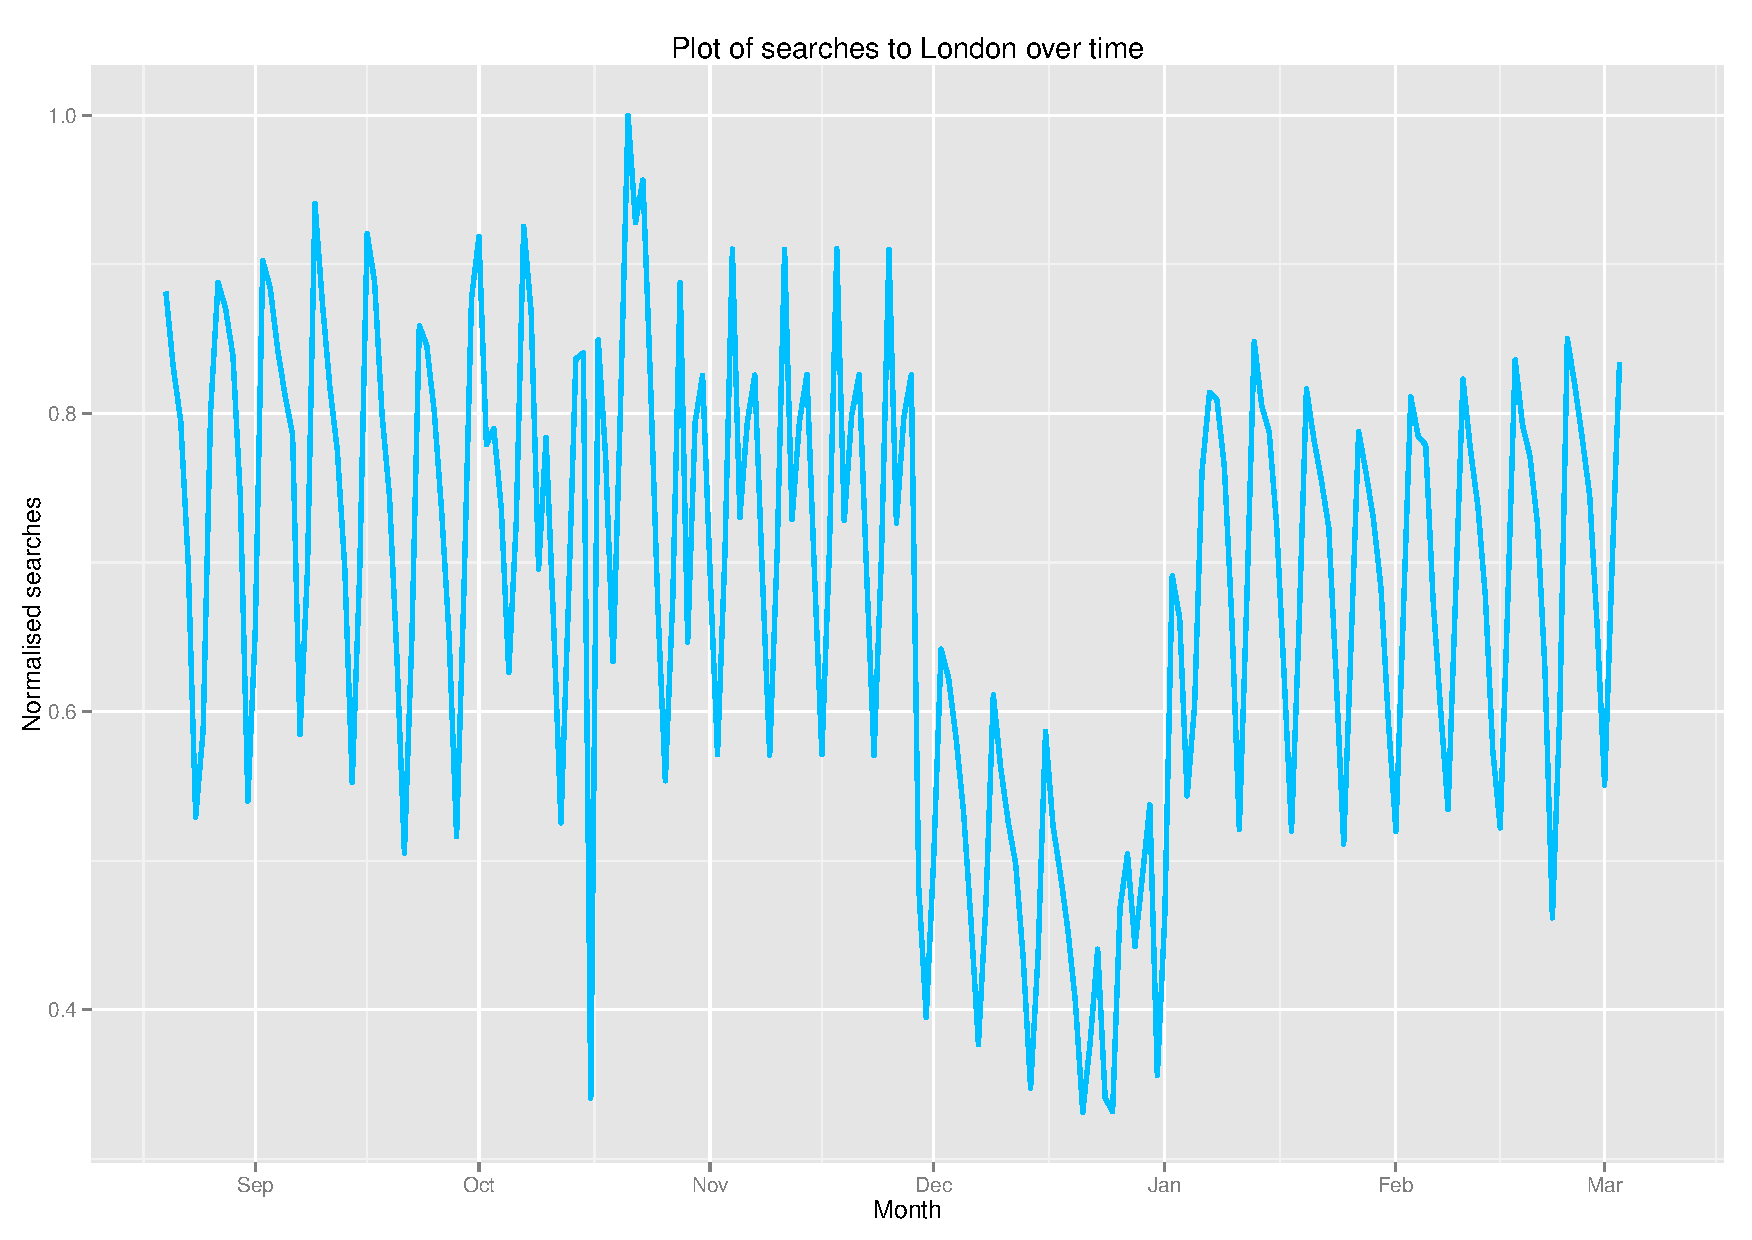
\includegraphics[scale=0.4]{london-searches}
\end{center}
\caption{Searches to London - as we can see the trundling is going to be almost parallel to the X axis.The slight dip in December is due to seasonality. That is noticed across the industry as a whole}
\end{figure}


\begin{figure}[]
\begin{center}
\includegraphics[scale=0.4]{ibiza-searches}
\end{center}
\caption{Searches to Ibiza - in this plot we can get the idea of seasonality. The dips is observed as soon as enter autumn and then in January the searches to such destinations pick up again as people are starting to plan their summer holidays}
\end{figure}

Naturally, because of the constant and not so changing nature of the first group, I would expect my model to perform better on the second group. The Root Mean Squared Error from my models on the 2nd group should be smaller or roughly the same as the error generated by the in-house algorithm. It's called  "Last 4 Fridays" and essentially it is a slightly tweaked version of an exponentially weighted moving average, which takes into account seasonality. A more detailed discussion as to why this was picked as the baseline can be found in Chapter \ref{sec:baseline} on page \pageref{sec:baseline}.


\section{Results for the first iteration of the algorithm}


In order to get started with this problem and generate a first set of results I had to identify a good way of modelling the problem and how to predict the output from some inputs. The first way of doing it suggested by my supervisor was to use LASSO \cite{lasso} in order to determine the weights for all of my inputs. 


The way the first iteration of my model works is the following - for every day you take the same day the week before, the week before that and so on for the last 4 weeks and you also take the Twitter counts for a destination as a feature as well. Instead of fixing their weights as in the in-house algorithm, I chose to let LASSO pick the weights for every feature. This way we get an incremental improvement over the Last 4 Fridays, that is taking into account one of the many exogenous factors that could influence the search volumes either upwards or downwards. I expected that to yield better results for the 2nd group of destinations and possibly for some from group 1. I will refer to the first iteration of the model as TwitterDF, where DF stands for dynamic Fridays. 


Overall, I was very pleasantly surprised by the results. On the full set of 1372 destinations, the first iteration of my model generated better predictions and had lower RMSE on 1034 of the destinations. On the other hand the in-house champion Last 4 Fridays performed better on 338 of the destinations. In order to illustrate that difference there is a scatter plot of the RMSEs in Figure 2.3. That means that my model is better on 75.3\% of all the destinations.

\begin{figure}[]
\begin{center}
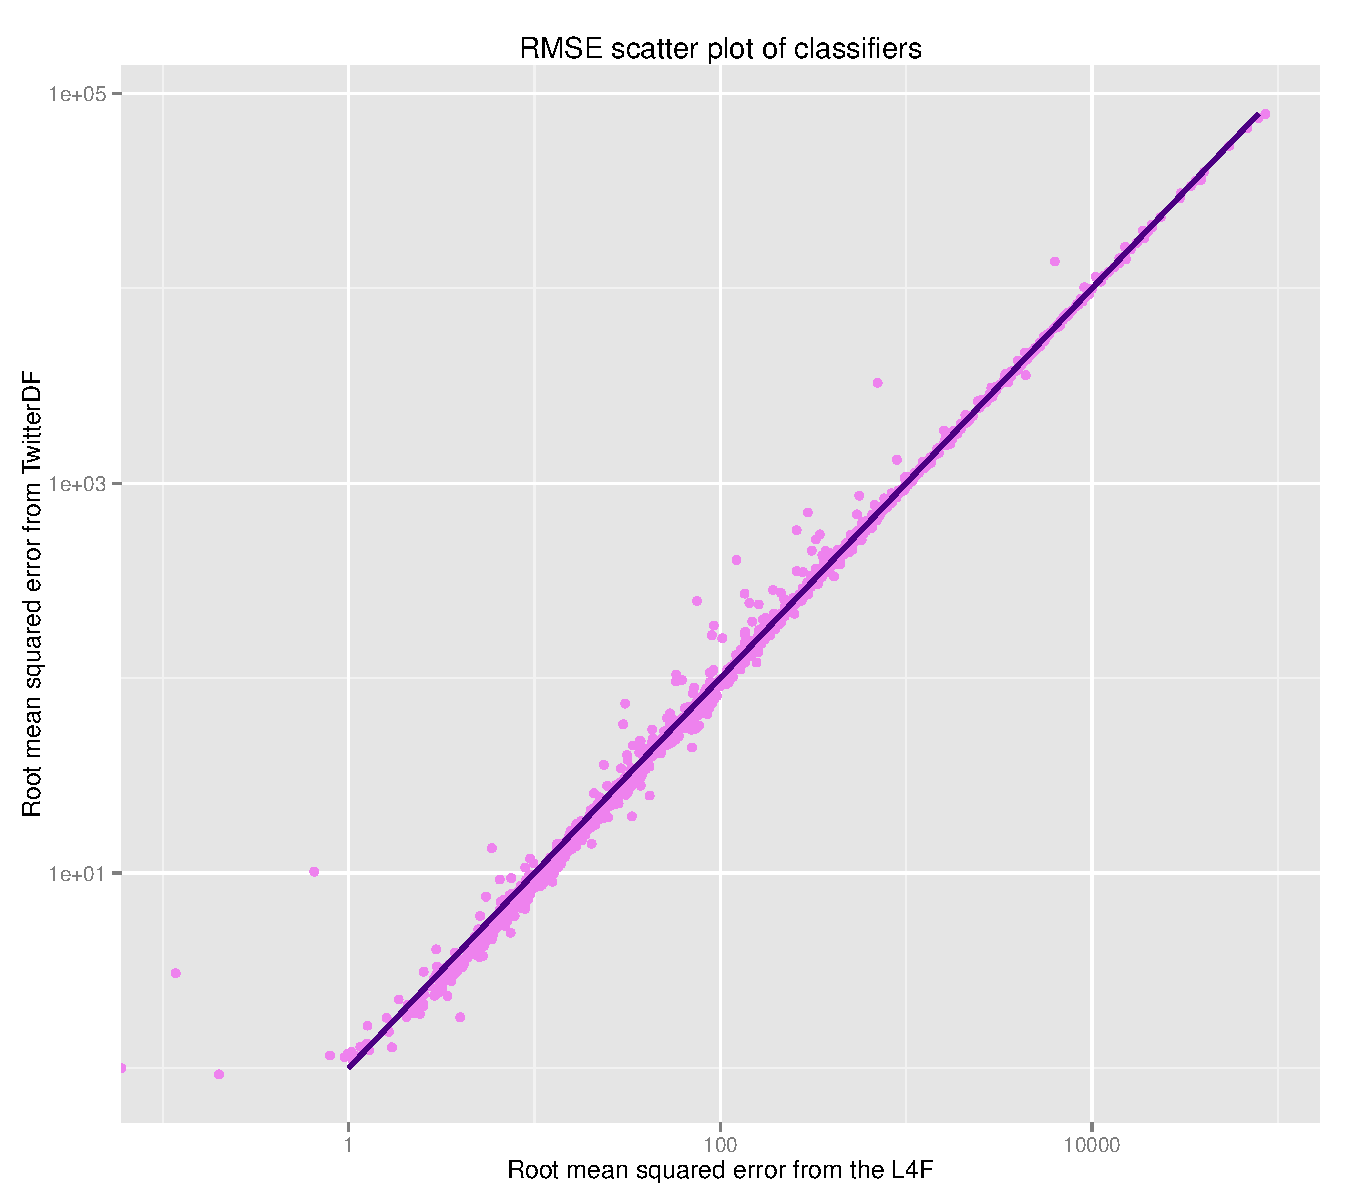
\includegraphics[scale=0.4]{RMSE}
\end{center}
\caption{Scatter plot of the RMSE of TwitterDF model and Last 4 Fridays. To put things into perspective, I've also plotted the y=x line to make it easier to visualise the border between the two. Anything below the line is where my model performs better and anything above L4F.  }
\end{figure}

In Figure 2.3 we can see that the performance of the the models is actually quite similar. Almost all of the dots are distributed along the x=y line. Contrary to my expectations that destinations from group 2 would be better classified by my model, actually it performs just as well on the more constant ones from group 1. 

In Table 2.1 and 2.2 you can find some picked which illustrate the worst performing models and best performing ones.

\begin{table}[]
\begin{center}
\begin{tabular}{ l | r | r | r}
Place & RMSE L4F & RMSE Twitter & Improvement \\
\hline
Parkersburg & 3.99 & 1.82 & 54.38\% \\
Bismarck & 33.41 & 19.53 & 41.54\% \\
Marshall Islands & 41.63 & 24.99 & 39.98\% \\
Cayo Coco & 70.44 & 44.10 & 37.38\% \\
Yakima & 7.44 & 4.94 & 33.65\% \\
Jonesboro & 3.40 & 2.34 & 31.11\% \\
Casper & 20.30 & 14.14 & 30.34\% \\
Barrow & 5.28 & 3.76 & 28.81\% \\
Niue & 12.50 & 9.02 & 27.82\% \\
Cedar City & 5.08 & 3.71 & 26.91\% \\
Sudbury & 8.89 & 6.56 & 26.24\% \\
\end{tabular}
\end{center}
\caption{Results for destinations that yielded the best improvement in percentage terms when classified with the model from this project in comparison to the in-house one. As we can see they are fairly small niche destinations where it seems that people tweeting about it likely to result in a flight search to that place.}
\end{table}

\begin{table}[]
\begin{center}
\begin{tabular}{ l | r | r | r}
Place & RMSE L4F & RMSE Twitter & Improvement \\
\hline
Hayman Island & 0.12 & 3.06 & -2511.33\% \\
Airlie Beach & 0.65 & 10.17 & -1456.42\% \\
Venezuela & 701.98 & 3277.16 & -366.85\% \\
Crooked Creek & 0.20 & 0.93 & -362.78\% \\
Pereira & 74.94 & 248.77 & -231.97\% \\
Launceston & 122.28 & 404.13 & -230.49\% \\
Jodhpur & 30.80 & 74.05 & -140.40\% \\
Manaus & 295.66 & 707.50 & -139.30\% \\
Del Rio & 5.89 & 13.42 & -127.63\% \\
Trondheim & 257.36 & 573.07 & -122.68\%
\end{tabular}
\end{center}
\caption{Results for destinations that yielded the biggest negative improvement. Quite an interesting mix destinations. The Venezula result is attributed to Venezuela trending lately, because of the civil uprisings. Eliminating such "negative" influences is one of my goals for next year.}
\end{table}


If we look at the top 10 destinations in terms of RMSE (and in flight searches) in Table 2.3 we see something quite surprising.  The improvement is positive in 9 out of the 10 examples. Even though it's small, the very fact that there is an improvement, means that taking into account exogenous factors is beneficial and can contribute positively to the quality of the prediction.

\begin{table}[]
\begin{center}
\begin{tabular}{ l | r | r | r}
Place & RMSE L4F & RMSE TwitterDF & Improvement \\
\hline
Spain & 85,844 & 78,424 & 8.64 \% \\
United States & 78,480 & 74,782 & 4.71\% \\
United Kingdom & 68,706 & 66,335 & 3.45\% \\
Italy & 54,804 & 53,780 & 1.87\% \\
London & 40,129 & 39,554 & 1.43\% \\
Russia & 38,712 & 36,033 & 6.92\% \\
Germany & 36,113 & 35,672 & 1.22\% \\
France & 34,020 & 33,393 & 1.84\% \\
Thailand & 29,997 & 30,701 & -2.34\% \\
Turkey & 29,616 & 28,912 & 2.38\% 
\end{tabular}
\end{center}
\caption{Results for the top destinations by RMSE of L4F. 9/10 have lower RMSEs with TwitterDF. As we can see for the top destination - Spain - the improvement is 8.64\%, which is great, because I expected the model to perform worse on places from group 1.}
\end{table}


\newpage
\section{Results for the 2nd iteration}

The 2nd iteration, was to fix the weights of the last 4 fridays and use the exponential weighting scheme that we have in the L4F model. I called that model TwitterCF where CF stands for compound Fridays. The scatter comparison for the two models is in Figure 2.4. In Table 2.4 is the overall comparison of which model has the lowest RMSE for how many of the total models. 

\begin{figure}[h!]
\begin{center}
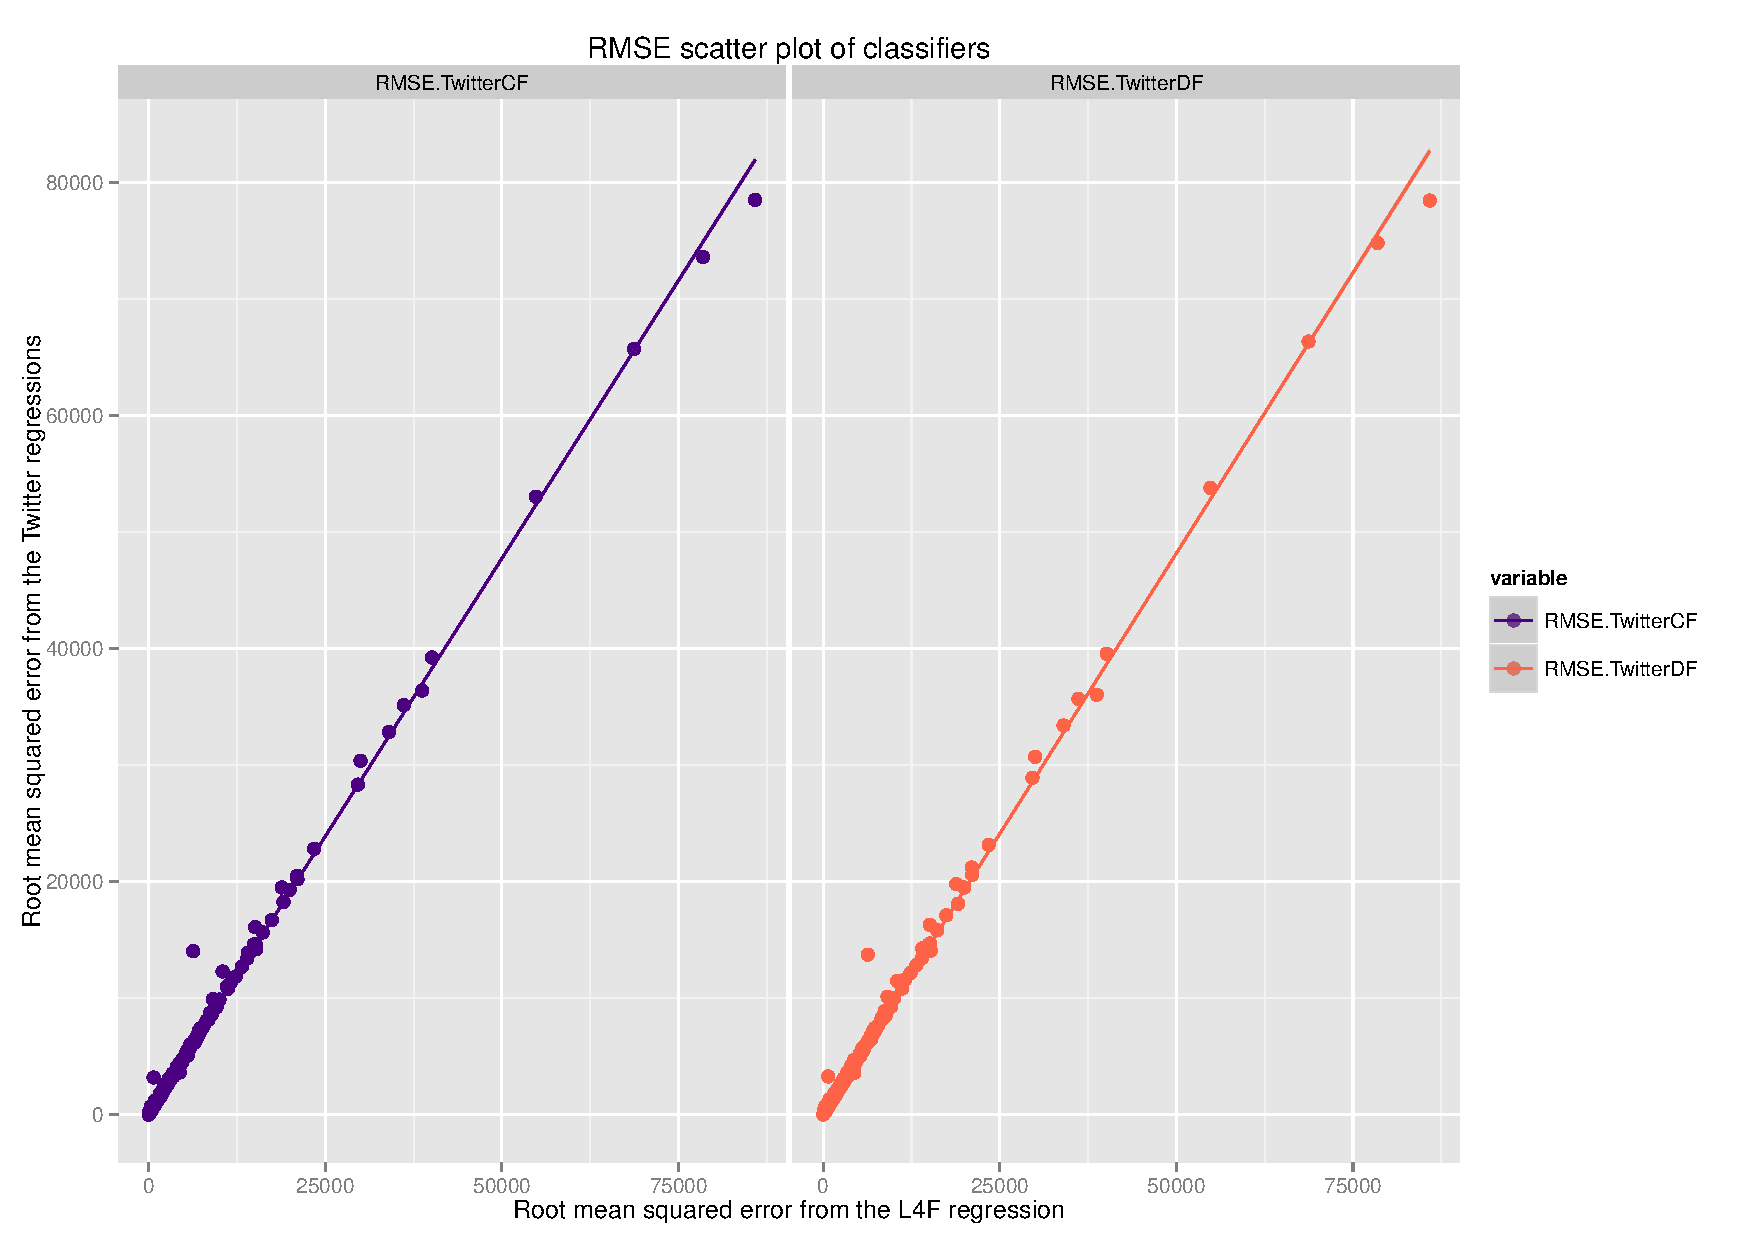
\includegraphics[scale=0.4]{rmse_scatter_by_reg}
\end{center}
\caption{The two models compared. TwitterCF stands for compound Friday - taking all of the previous Fridays with predetermined weights and using them as a single weight in the regression. TwitterDF is leaving everything to LASSO.}
\end{figure}

\begin{table}[h!]
\begin{center}
\begin{tabular}{ l | r }
Method & NumBest \\
\hline
L4F & 226 \\
TwitterCF & 741 \\
TwitterDF & 405 \\
\hline
\textbf{Total} & \textbf{1372}
\end{tabular}
\end{center}
\caption{Comparison of the three methods and who had the best results on the dataset of 1372 points. As we can see, the Twitter models have got a definite majority. 83\%+ of the results have the lowest RMSE with the Twitter models}
\end{table}

In Table 2.5 you can find a more detailed breakdown of the top 20 destinations by RMSE for L4F sorted descending. It includes the improvement of the Twitter models and the improvement of the CF model over the DF one. Overall, the average improvement of the CF model is 0.96\% across all the 1372 individuals models for every destination.

\begin{table}[p]
\begin{center}
\begin{tabular}{ l | r | r | r | r | r | r }
Place & L4F &  TwitterCF & TwitterDF & Best & Improv. & CF/DF Imp. \\
\hline
Spain & 85,844 & 78,485 & 78,424 & TDF & 8.64\% & -0.08\%\\
US & 78,480 & 73,581 & 74,782 & TCF & 6.24\% & 1.61\%\\
UK & 68,706 & 65,696 & 66,335 & TCF & 4.38\% & 0.96\%\\
Italy & 54,804 & 53,020 & 53,780 & TCF & 3.26\% & 1.41\%\\
London & 40,129 & 39,222 & 39,554 & TCF & 2.26\% & 0.84\%\\
Russia & 38,712 & 36,375 & 36,033 & TDF & 6.92\% & -0.95\%\\
Germany & 36,113 & 35,137 & 35,672 & TCF & 2.70\% & 1.50\%\\
France & 34,020 & 32,816 & 33,393 & TCF & 3.54\% & 1.73\%\\
Thailand & 29,997 & 30,374 & 30,701 & L4F & -1.26\% & 1.07\%\\
Turkey & 29,616 & 28,316 & 28,912 & TCF & 4.39\% & 2.06\%\\
Greece & 23,423 & 22,810 & 23,144 & TCF & 2.62\% & 1.44\%\\
Australia & 21,072 & 20,189 & 20,573 & TCF & 4.19\% & 1.86\%\\
New York & 21,026 & 20,498 & 21,198 & TCF & 2.51\% & 3.30\%\\
Paris & 19,966 & 19,287 & 19,492 & TCF & 3.40\% & 1.05\%\\
Barcelona & 19,087 & 18,237 & 18,093 & TDF & 5.21\% & -0.80\%\\
Bangkok & 18,831 & 19,496 & 19,783 & L4F & -3.53\% & 1.45\%\\
Portugal & 17,429 & 16,694 & 17,103 & TCF & 4.22\% & 2.39\%\\
Netherlands & 16,146 & 15,638 & 15,816 & TCF & 3.14\% & 1.12\%\\
China & 15,212 & 14,188 & 14,074 & TDF & 7.48\% & -0.81\%\\
Istanbul & 15,121 & 14,642 & 14,692 & TCF & 3.16\% & 0.34\%
\end{tabular}
\end{center}
\caption{Comparison of the RMSE generated by the 3 models for the first 20 destinations with highest RMSE for L4F. The Best column indicates who has the lowest RMSE for that destination. Out of the twenty TwitterDF and TwitterCF perform better on 18 of the destinations. The overall numbers can be found in table 2.4. The average improvement of CF over DF is 0.96\%, which even though small is significant nonetheless. }
\end{table}

%\section{Results when shifting by one day}

\newpage
\section{Results for the algorithm with more features}

In the next iteration of the model I didn't limit it to just twitter counts and searches from previous dates. For this particular model I've used all the words co-occurring with a place name as features. Of course, there is a lot of junk, so I removed all the emoji characters and all the stop words in order to prevent overwhelming the LASSO with a lot of junk features.

In Table 2.6, 2.8 you can see the results from the extended model on Tenerife and Sochi. In the tables you can see the improvement in RMSE for Twitter and the decrease in the number of features with non-zero weights. For both of those destinations, the Twitter models perform better for some values of the penalisation parameter $\alpha$. I've picked them, because they are both really interesting - for Tenerife L4F start well, then Twitter has lower RMSE, but as we discard more and more features, L4F wins again. Sochi was picked because of the olympics, which has massively affected the number of searches to Sochi (increase of about 10 times), but the number of tweets about Sochi has gone up as well. 
It's also quite interesting, because of local minima of RMSR, where it decreases and then picks up again.

\begin{table}[h]
\begin{center}
\begin{tabular}{ l | r | r | r | r | r | r}
$\alpha$ & $>$ 0 W CF & RMSE TCF & $>$ 0 W DF & RMSE TDF & RMSE L4F & Best\\
\hline
0.50 & 191 & 11,683 & 200 & 14,961 & 1,517 & L4F\\
1 & 175 & 12,507 & 177 & 15,647 & 1,517 & L4F\\
2 & 146 & 13,288 & 151 & 15,161 & 1,517 & L4F\\
5 & 136 & 13,607 & 131 & 14,387 & 1,517 & L4F\\
10 & 116 & 12,728 & 114 & 11,341 & 1,517 & L4F\\
20 & 112 & 11,379 & 108 & 8,950 & 1,517 & L4F\\
50 & 88 & 6,601 & 85 & 5,197 & 1,517 & L4F\\
125 & 51 & 1,946 & 56 & 2,009 & 1,517 & L4F\\
250 & 33 & 1,684 & 36 & 1,788 & 1,517 & L4F\\
\hline
500 & 22 & 1,596 & 23 & 1,465 & 1,517 & TDF\\
1,000 & 11 & 1,423 & 13 & 1,593 & 1,517 & TCF\\
2,000 & 5 & 1,356 & 8 & 1,815 & 1,517 & TCF\\
4,000 & 1 & 1,366 & 4 & 1,854 & 1,517 & TCF\\
8,000 & 1 & 1,366 & 4 & 1,853 & 1,517 & TCF\\
16,000 & 1 & 1,366 & 4 & 1,852 & 1,517 & TCF\\
32,000 & 1 & 1,366 & 4 & 1,850 & 1,517 & TCF\\
\end{tabular}
\end{center}
\caption{Improvement in RMSE for Tenerife. As we can see after we get to a certain point the Twitter models get better and better, until it gets to discarding all of the weights, but the Fridays. The optimal result for Twitter CF is with 5 weights, since the reduction in RMSE afterward is negligible, while the DF version performs best with 23 and it starts getting worse. The features and weights at $\alpha = 1000$ are in Table 2.7}
\end{table}

\begin{table}
\begin{center}
\begin{tabular}{l | r}
Feature & Weight \\
\hline
time & 583.35 \\
\#tenerife & -87.43 \\
\#solareclipse & 35.74\\
tenerife & -19.29\\
friend & 64.81\\
Fridays & 0.75\\
begins & -30.50\\
heres & 7.72\\
would & -273.96\\
canary & -7.56\\
view & -10.86 \\
\end{tabular}
\end{center}
\caption{Weights for Tenerife at $\alpha=1000$. These are the weights that the TwitterCF model has picked.}
\end{table}

\begin{figure}[]
\begin{center}
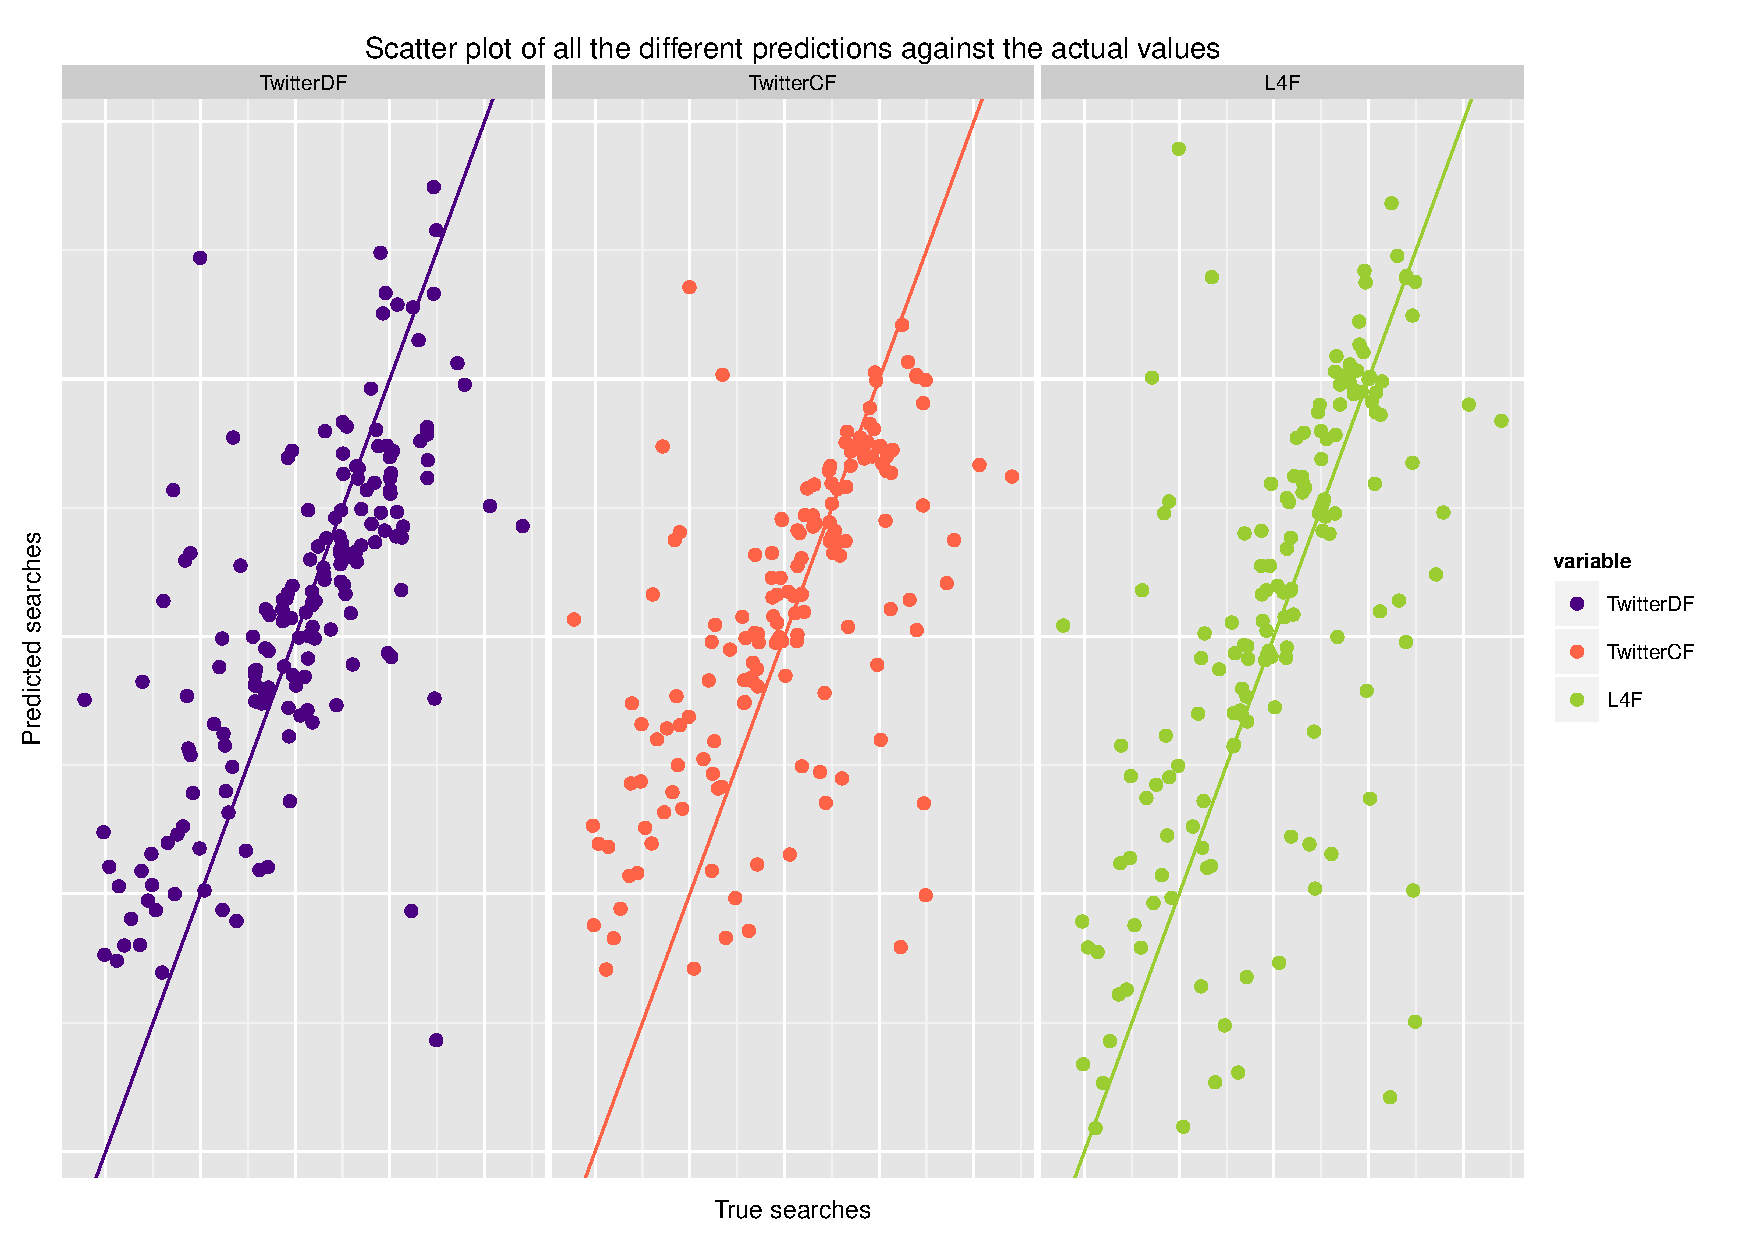
\includegraphics[scale=0.5]{plots/Tenerife}
\end{center}
\caption{Predictions vs actual for a destination from group 2 - Tenerife. For this group Twitter models make actual gains, albeit small.}
\end{figure}

\begin{table}[h!]
\begin{center}
\begin{tabular}{ l | r | r | r | r | r | r}
$\alpha$ & $>$ 0 W CF & RMSE TCF & $>$ 0 W DF & RMSE TDF & RMSE L4F & Best\\
\hline
0.5 & 268 & 10,545 & 377 & 15,909 & 9,156 & L4F\\
1 & 200 & 10,505 & 260 & 15,108 & 9,156 & L4F\\
2 & 170 & 9,976 & 192 & 13,693 & 9,156 & L4F\\
\hline
5 & 138 & 8,774 & 158 & 10,720 & 9,156 & TCF\\
10 & 126 & 8,964 & 132 & 9,808 & 9,156 & TCF\\
20 & 112 & 9,051 & 115 & 10,802 & 9,156 & TCF\\
50 & 99 & 8,867 & 101 & 9,577 & 9,156 & TCF\\
125 & 81 & 9,129 & 82 & 8,604 & 9,156 & TDF\\
250 & 60 & 8,924 & 57 & 8,304 & 9,156 & TDF\\
500 & 41 & 8,335 & 44 & 7,982 & 9,156 & TDF\\
1,000 & 29 & 8,443 & 28 & 8,164 & 9,156 & TDF\\
2,000 & 16 & 8,424 & 19 & 8,341 & 9,156 & TDF\\
4,000 & 7 & 9,143 & 9 & 9,307 & 9,156 & TCF\\
\hline
8,000 & 3 & 9,759 & 6 & 9,938 & 9,156 & L4F\\
16,000 & 2 & 9,727 & 5 & 9,860 & 9,156 & L4F\\
32,000 & 2 & 9,950 & 4 & 10,010 & 9,156 & L4F\\
\end{tabular}
\end{center}
\caption{Improvement in RMSE with the expanded feature set for Sochi, which is in 2nd group of destinations.  
As you can see in terms of absolute value, the RMSE for the Twitter model with compound fridays - RMSE TCF - has decreased 20\% for the area where TCF has the lowest RMSE. I have separated the area where the Twitter Models are better with two horizontal lines. The RMSE for TDF is 2 times lower at $\alpha=500$ and that's where the model performs the best. Both models have a comparable number of weights, which is really interesting. The weights for  }
\end{table}

\begin{table}
\begin{center}
\begin{tabular}{l | r}
Feature & Weight\\
\hline
team & 16.08\\
\#olympics2014 & 2.40\\
Count & 1.34\\
olympic & 1.30\\
Friday1 & 0.75\\
canada & 0.72\\
Friday3 & 0.16\\
Friday2 & 0.11\\
Friday4 & -0.15\\
hotel & -1.07\\
\#seeyouinsochi & -1.22\\
jump & -1.49\\
\#olympics & -2.24\\
dog & -2.56\\
sochi & -2.52\\
\end{tabular}
\end{center}
\caption{Handpicked features for Sochi at $\alpha=500$. The total number of features is 44 and they are the ones picked by TwitterDF. Interestingly enough dog, sochi and hotel very negative weights. On the other hand there are a few positive weights that relate to the olympics.} 
\end{table}



\begin{figure}[]
\begin{center}
\includegraphics[scale=0.4]{plots/Sochi}
\end{center}
\caption{Predictions vs actual for a destination for Sochi. The olympics made any pattern in the data very hard to spot.}
\end{figure}

As we can see the more the junk features are penalised the classification improves. However that is still just the beginning. Next year I will apply more NLP on the Twitter dataset trying to capture only the relevant tweets that will result in an improvement of the overall RMSE for the classifier. 


\begin{figure}[p]
\begin{center}
\includegraphics[scale=1.0]{Sochi}
\end{center}
\caption{Searches and tweets to Sochi. The massive spike is around the Olympics. As we can see the two time series are correlated and the spike it tweets is just a bit before the spike in searches.}
\end{figure}


However those gains are not observed across the whole board at all. In table 2.11 are the results for the United Kingdom. Even though we notice a  very significant improvement, the results are still poorer than L4F. Of course, there are still 14 and 11 weights in both models, so we could continue increasing the penalisation factor further, but that would turn tweaking and tuning the classifiers into a very complicated and laborious task and of course we will get into the problem of overfitting.

\begin{table}[h!]
\begin{center}
\begin{tabular}{ l | r | r | r | r | r | r}
$\alpha$ & $>$ 0 W CF & RMSE TCF & $>$ 0 W DF & RMSE TDF & RMSE L4F & Best\\
\hline
0.5 & 583 & 60,924 & 649 & 70,068 & 8,700 & L4F\\
1 & 467 & 65,234 & 523 & 68,728 & 8,700 & L4F\\
2 & 369 & 65,253 & 412 & 76,945 & 8,700 & L4F\\
5 & 280 & 59,667 & 290 & 69,158 & 8,700 & L4F\\
10 & 231 & 54,972 & 241 & 62,057 & 8,700 & L4F\\
20 & 197 & 58,161 & 212 & 55,629 & 8,700 & L4F\\
50 & 167 & 62,001 & 175 & 77,956 & 8,700 & L4F\\
125 & 147 & 59,146 & 155 & 90,270 & 8,700 & L4F\\
250 & 139 & 73,864 & 142 & 105,197 & 8,700 & L4F\\
500 & 116 & 81,806 & 120 & 96,173 & 8,700 & L4F\\
1,000 & 106 & 84,796 & 110 & 91,576 & 8,700 & L4F\\
2,000 & 98 & 61,891 & 94 & 60,692 & 8,700 & L4F\\
4,000 & 71 & 44,306 & 68 & 61,037 & 8,700 & L4F\\
8,000 & 44 & 56,021 & 43 & 49,030 & 8,700 & L4F\\
16,000 & 27 & 31,209 & 29 & 28,339 & 8,700 & L4F\\
32,000 & 11 & 15,895 & 14 & 16,034 & 8,700 & L4F\\
\end{tabular}
\end{center}
\caption{Both TwitterDF and CF decrease the number of features significantly the RMSE for both is about 2x times the one for L4F.}
\end{table}


\newpage
\section{Results on the full dataset}

%\subsection{With just Twitter counts}

Another interesting benchmark was how it performs on the overall search volumes. In Table 2.11 you will find how the two models perform on the all the Twitter counts summed together and the searches to all of those destinations.

\begin{table}[h!]
\begin{center}
\begin{tabular}{ l | r | r | r | r}
 & RMSE TwitterDF & Twitter CF & RMSE L4F & Difference \\
\hline
Overall & 1,640,111 & 1,621,391  & 1,674,130 & 3.1 \% \\
\end{tabular}
\end{center}
\caption{RMSE on the tweet counts for all destinations and searches to all destinations. Difference is the percentage improvement of the best of the twitter models.}
\end{table}

As you can see in Figure 2.8 the overall volume of searches is not as volatile as the destinations in group 2, so it would fall into group 1, but surprisingly enough the Twitter models do a marginally better job at predicting.

\begin{figure}[h]
\begin{center}
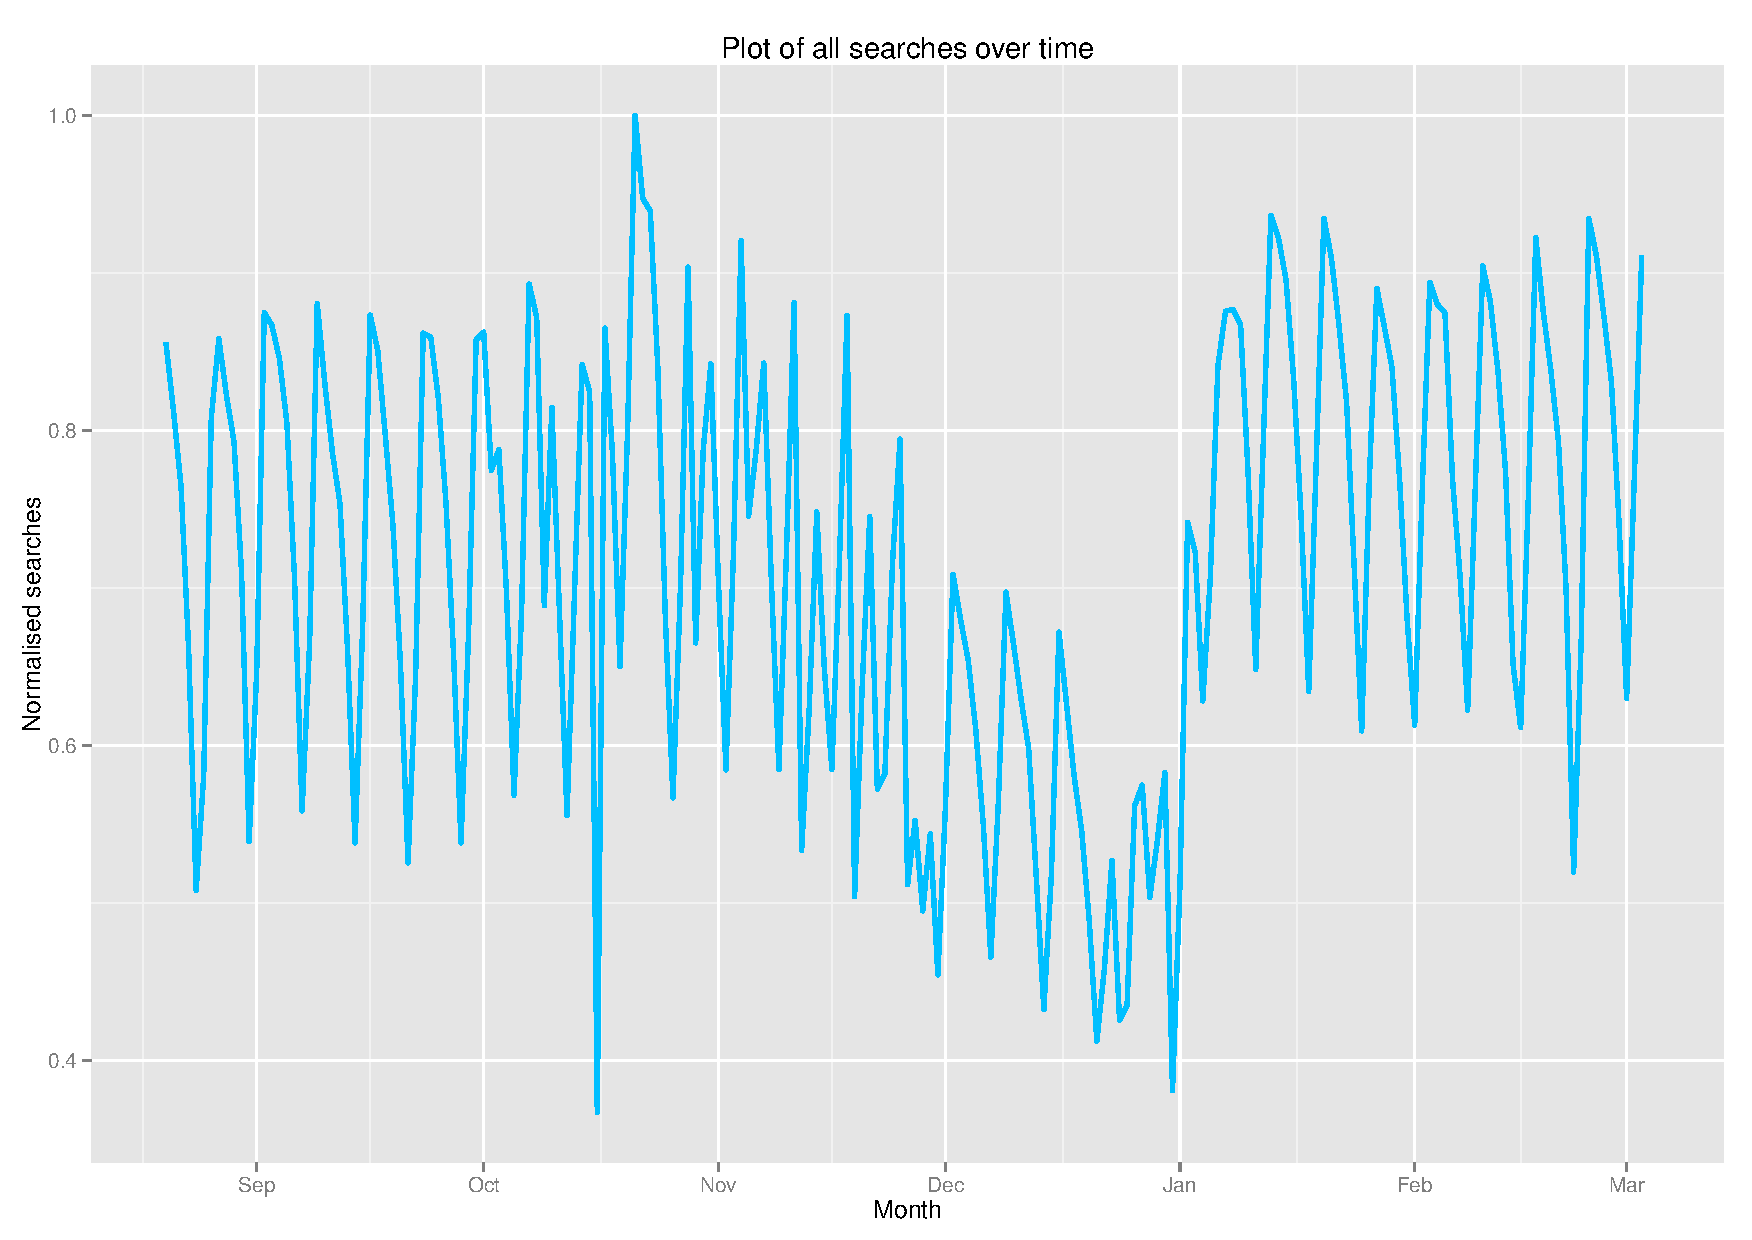
\includegraphics[scale=0.4]{overall}
\end{center}
\caption{Plot of all the searches to all the destinations. This would fall into the first group of steady constant volumes}
\end{figure}

%\subsection{With more features}
%
%Here
\newpage
\section{Conclusion}

The previous results have demonstrated that there is definitely a gain, even though not as great as I expected, in including exogenous factors such as Twitter in the prediction. With the first level of filtering described in chapter \ref{sec:tweettext} on page \pageref{sec:tweettext} we have achieved better prediction on slightly more than 83\% of all the destinations.  


During the 2nd phase of the project, I will focus on retrieving only the most relevant tweets from the Twitter dataset and doing better feature extraction that will allow to remove junk features that bring the RMSE up. With that in mind, I am hopeful that I will be able to build the next version of the model that is going to perform just as well on the first group of destinations. 



\chapter{Background and discussion of related work}


With millions and some with billions of users, Social Networks are becoming an increasingly more important in our lives. A big proportion of people use it as their primary way of communicating with the outside world - people will "tweet" about anything, post to Facebook, check in on FourSquare, instagram their food and so on. We have become perfectly fine with externalising our lives and posting every minute detail about our lives online and thusly making it available to everyone else. 
Of course, there are always exceptions. After all 82\% of the world's population are not on Facebook, but those 1.23 billion monthly active users are all using it. Not all of them are avid users and post all of their pictures to it, but a big proportion is. With this amount of data on one's behaviour, life patterns and activities, companies can build a very good understanding of every individual. 


As with any other network - be it TV, radio, newspaper - there are always going to be some who are trying their best to commercialise it and benefit from it in some way. Since people are willing to share so much information about themselves online, there are terabytes of data being generated every day on what people did, what things they tweeted about, their latest pictures, etc. As we are entering the "Big Data" age where every company is trying to turn its data into a product or simply establish itself as the leading data supplier for a particular market. Due to the vastness and volumes of the data that these social networks generate they have sprung an entirely new eco-system of its own - companies are now plugging into Twitter, Facebook and all the other networks to figure out everything they can about you. Everyone is now talking about "sentiment analysis" in social media for brands, targeting particular demographics with ads on Facebook, promoting tweets and segmenting the customers into different groups and selling their data to marketers.


A particularly interesting one of that new generation of networks is Twitter. With a base of 200+ million active users it has slowly but surely become one of the most prominent sources of information and news on the web. It's previously beaten traditional news sources on numerous occasions by a few minutes when delivering the latest developments such the Los Angeles earthquake in 2008. \cite{TwitterNewsWire} They have their data streams opened up to developers and researchers as well, which is a fantastic opportunity to mine this data set for valuable information. There are plenty of articles on the internet on what people have done with it - demographics research, predicting flu outbreaks, etc. \cite{TwitterResearch} Miles Osborne here at the University of Edinburgh has done quite a lot of research using the Twitter data streams  \cite{Miles} and perhaps the biggest use is in Sasa Petrovic's PhD thesis. \cite{Petrovic2012}


In order to get more familiar with the trending events I have done read a few papers on Topic Detection and Tracking and First News Detection in order to see if I could use and extend it for my case. I'd like to mention Sasa Petrovic's PhD thesis as an excellent paper on the matter. \cite{Petrovic2012} However after careful investigation into the complexity of TDT I decided that this will be implemented in the 2nd part of the project, since I needed to familiarise myself with the dataset, try to see if there is more intelligent filters on the data stream and see how exactly they can be correlated to my 2nd dataset.


As it's been said many times "Predicting is hard, especially about the future".  Add a noisy channel as a source of input and one is only making things worse. There have been several attempts to predict something based on Twitter - stock markets \cite{twitstock},  flu outbreaks \cite{twitflu}, results for the NFL \cite{twitnfl} and poll results \cite{twitpoll} being the most prominent published papers.


In order to predict the stock markets \cite{twitstock}, the authors try to use the cutting edge of the real-time twitter data in order to classify the overall mood and from that to predict whether the DIJA \cite{dija} is going to go up or down. In order to achieve it they use OpinionFinder \cite{opfind}, which can measure opinion classifying it into negative or positive. To capture the complexity of human moods, they created their own system called GPOMS, which can capture up to 6 states. 
In order to make the OF and GPMOS time series comparable, they used their z-scores. They have proven that the GPOMS values are more descriptive of public moods than the OF binary sentiment. However correlation does not imply causation and in order to check whether there is any they use the Granger causality analysis \cite{granger}. It rests on the assumption that if X causes Y then changes in X will systematically occur before changes in Y. However in this case they are not testing whether there is actual causation, but rather there is predictive information in the public mood time series that can describe the time deltas in DIJA. Out of all the different mood values Calm has the highest predictive value. After determining that there is definitely a gain in using the Calm values to predict the DIJA delta they use a Self-Organising Fuzzy Neural Network (SOFNN) \cite{sofnn}, which is a five-layer hybrid neural network, which has the ability to organise its neurons during the learning process by itself. After tuning and predicting the values on their dataset, they confirmed that Calm has the best predictive value. 

However, in their discussion they not that they are not really filtering their users on any particular geographical, language or cultural level. In this project, we have only taken \emph{tweets} from the United Kingdom, which allows us to try to predict where people from the UK want to fly to. As far as their methods are concerned, working with Neural networks is certainly one of the options that I'd like to investigate next year, but because of the fine tuning and additional overhead of using and training and possibly implementing it, I decided to leave this more complicated method for next year. 


On the other hand you can do simpler things when you are trying to predict public opinion on a certain topic \cite{twitpoll}. The authors make a strong argument that using Twitter you can replace the expensive time inefficient polls. They use public sentiment in order to predict ups and downs in the consumer confidence rating. In order to remove any massive outliers and because of the volatile nature of public sentiment they use something they call "Moving average aggregate sentiment", which smoothers out the daily variations. For the classification and prediction they use a Linear Least-Squares model with a lag hyper parameter. The hyper parameter is a good idea for my projects and it's certainly a very good option to explore, because sometimes the public might not go out and search flights straight away, but instead do it the next day. That is certainly something that should be considered when building the models later.


Of course Twitter can be used to predict other things with some success as well - NFL games \cite{twitnfl} or general state of public health. \cite{twitflu} In \cite{twitnfl} they have used Canonical correlation analysis (CCA) to combine the Twitter features with the statistical game features and to maximise the correlation of the combined features. With that method they get about 50\% prediction accuracy. 


In \cite{twitflu} the very fact that a big proportion of Twitter's 200 million monthly users is used to paint a picture on public health in the US. They discuss the limitations of twitter and the fact that due to geocoding limitations, they couldn't provide a more specified per user analysis, but overall the correlations in the paper are astonishing and show the breadth that Twitter data gives. 


In the aforementioned papers I have shown the different ways in which Twitter could be used to predict something about the future. Since people are inclined to post a lot of information on it, why wouldn't we be able to do something something specific in a more niche area like predicting search volumes?


Using Twitter for research has been quite an active area, because of its amazing breadth and the amount of data one can extract and process.
On the other hand, the only thing that has been researched in the online travel sector is what is the optimal time to book an airline flight. \cite{Hamletkdd03} \cite{ijcai} In order to do it one has to consider a lot of factors, because human action can cause massive shifts in those prices very easily. 
Both of the referenced papers are using small sets of data which aim to predict what is the optimal time to book. What is written there is the other part of the puzzle - when should you book, but in this particular project we are more interested in when ARE people looking for flights.


The Methodology can be found in chapter \ref{chap:method} on page \pageref{chap:method} split by all the main subtasks that had to be carried out. The subtasks are described in detail and each one of the sections includes an overview of what was done, how it was done and what difficulties were encountered and how I overcame them. 


Chapter \ref{chap:model} on page \pageref{chap:model} explains what are the Machine Learning models used to carry out the work for this project. Since there is no model defined anywhere I had to use an in-house algorithm used by Skyscanner to predict the search volumes. It's then described in depth which model worked best and why. 


In chapter \ref{chap:future-work} on page \pageref{chap:future-work}, I discuss all the future work that will be carried out for this project both for next year and if someone is to pick it up and start developing on top. In order to do that I have included links to the source code for this project and all the pre-aggregated data sets from Twitter in the repository.



\chapter{Methodology}
\label{chap:method}


As said earlier, this problem is something that no one has researched before. The lack of previous work and little to none understanding of how to approach this problem gave a lot of room to manoeuvre, but it was also very hard to see whether I am on the right track.


In order to get started with the whole project I thought that the most logical first step would to explore both of my datasets. Since that is quite a fuzzy term I wanted to see what information both of them hold and what I can extract. As far as the searches data set was concerned, since I have been an employee of Skyscanner for some time, I knew exactly what the data is, what it means and I could spot when a number just felt wrong. So the Skyscanner dataset did not require any extra effort from me. 


Twitter on the other hand was a challenge. The task of exploring the data was far from trivial, just because of the sheer size. The Sample stream (1\% of all tweets) which I used \cite{samplestream} was returning around 6 GBs of data a day, which is not small by any means. With some filtering and picking all the relevant attributes, I decreased the level of data to 3.5 GBs a day. I have described in detail the attributes I picked for this project section in \ref{sec:dc} on page \pageref{sec:dc}. That is roughly half of the original input, but that is the data I receive on a daily basis. As of the time of writing I have gathered about 500 GBs of data in total, which equals roughly around 550 million tweets. Since this is not an issue one encounters every day, I had to be very careful on how I structure my system in order to make sure it is as robust as possible and it's not going to buckle under the volumes of data coming in for processing. 

That left me with a few challenges, which were crucial to the success of this project:
\begin{enumerate}
\item How do I traverse the data in an efficient and clever without overdoing myself or performing unnecessary computation? That meant that I needed to store all the processed data in a way that it's easy to add the data as it comes.
\item What are the appropriate data structures in which I can hold the data, so they are easily transferable onto other parts of my system? For instance what would the data flow be from collection to preparation and then to the models.
\item How do I build a scalable and performant system for data analysis of the tweets, that will allow me to perform experiments in a easy and reproducible fashion?
\end{enumerate}

All of these challenges have made me spend a roughly about 100 hours in designing, building and testing the system that performs all of the computation. All of the code can be found in the code repository on GitHub \cite{code}. The codebase includes separate classes which filter the data, process it and convert it to time series, combine the two datasets together and then perform the regression. That is roughly the flow for the first iteration of the model that uses just Twitter counts and search data. The 2nd iteration also uses as many features as possible, so it has a separate class, which process the filtered data and extracts all the relevant features for a particular destination. All of the data filtering is described in detail in part  \ref{sec:dp} on page \pageref{sec:dp}. The main aim of the filtering is to take the 500GB dataset of tweets and take only the relevant ones, making a small working set, which can reside on a local SSD, which enables very fast processing and aggregation, which is then fed into the model for the regression and evaluation. 

In this chapter I will describe in detail every one of the main parts of the way I went from just gathering data to a full system for analysis and visualisation of the data and also how I solved any problems that I encountered.

%I have shown what I am using and how I process the data in \ref{sec:dp} on page \pageref{sec:dp}. My implementation was fast enough, because of the reduction to a smaller working set and it was able to process the whole reduced dataset in about 20 minutes, which is fast enough for re-processing.
%After collecting and preparing the data comes the next big question - what do I want to get out of this set? I have tried two ways of filtering it and trying to use it to predict the flight searches:
%\begin{itemize}
%\item Using hashtags which contain a country or city name and taking their counts.
%\item Taking every tweet that has a city/country name in its text in a conduction with a travel related term from the list. 
%\end{itemize}
%Both of these methods have obvious advantages and disadvantages - taking only hashtags will be really fast, but not expressive and representative enough. They are both explored in  \ref{sec:hashtag} and \ref{sec:tweettext} respectively. 
%Before building the models there was a final step that had to be done and that was cleansing the data. Because of some teething issues with problems with the Skyscanner data and the fact that the data collections process is not perfect, there are some holes in the data. 
%For the Skyscanner data set I have used the Last 4 Fridays forecasting method to backfill and for Twitter I've just used the means to fill in the missing values. 

\section{Data collection}
\label{sec:dc}


The first and most important set to any Machine Learning project is to collect all the data you can. In my case I had two different sets I had to work with - the data flowing in from the Twitter Public Stream and the search data coming in from Skyscanner. As said previously the data from Skyscanner didn't need any additional work in terms of familiarising myself, because I could easily pull it out with a SQL script and give myself all the necessary aggregations without any problem. 

The first and most important part of this project was to start collecting the correct data, which was to be used in building the model later. Twitter offers quite a comprehensive API with a lot of attributes, however in order to reduce the daily volume of data I had to take the most relevant ones for me. 


\begin{table}[p]
\begin{center}
\begin{tabular}{ l | p{11cm} }
Attribute & Explanation \\
\hline
Text & the text of the tweet is the most important one, perhaps. Quite a lot of information can be extracted from it alone \\
Id & the tweet id. Useful if we want to screen scrape for any additional information or just to provide a tidy small dataset of ids. \\
ID Str & String representation of the above. \\
Source & What is used to post the tweet. The Twitter website is marked as "web". \\
Coordinates  & Representation of the geographical location of the Tweet as reported by the utility used to post the tweet. \\
Entities & This include hashtags, user mentions and urls included in the tweet. Could be taken from the text, but it's nicer to have them ready. \\
Retweet count & the number of times the tweet was retweeted. Useful for any future models.  \\
Favourited & Indicates whether the tweet was favourited by people - an analogy of this would be a Facebook like.  \\
Language & The language of the tweet. We are capturing English language tweets at the moment, but put in place for future expansion into the multi-language domain  \\
Filter level & indicates the level of filtering applied to the stream. \\
Place &  Shows where the tweet was tweeted from. Gives more detail than coordinates - country, city name, coordinates as well. Not necessarily available for all tweets. \\
\end{tabular}
\end{center}
\caption{Attributes chosen to capture.}
\end{table}

The first stage of the project is to look only at tweets in English coming from the UK. That will allows us to predict and model the flight search volumes in the UK based on the mentions in the Twitter Stream.

The second stage would be to develop the model even further and add multi-language and multi-country support and employ more sophisticated models such as ARIMA or Auto-regressive Vector Models.

By selecting those particular tweet attributes and using the Streaming API, I managed to reduce the daily volume of data from \textasciitilde 6GB of data down to \textasciitilde 3.5GB/day.
The amount of data accumulated at the time of writing is \textasciitilde 380 GB. The collector has been running successfully from September 2013, however there are some holes of the data caused by network outages or the script interacting with the Twitter Streaming API crashing. 

The data on flight search volumes is kindly provided by Skyscanner. In order to ensure that there are no concerns with confidentiality I have anonymised the data. 

\section{Data processing}
\label{sec:dp}

\section{Hashtags}
\label{sec:hashtag}

Hashtag is one of the most important constructs by Twitter. Here's an example tweet:

\begin{quotation}
@FunnyChap: Something witty and very well said \bf{\#jokeoftheweek}
\end{quotation}

The structure of the tweets is:
\begin{enumerate}
\item The name of the user is denoted with a @ before the username.
\item The text itself.
\item The hashtag (a special Twitter construct) is denoted with a \#.
\end{enumerate}

You can filter out and explore twitter content based on hashtags and usually every major event has its own hashtag. The ones which are most mentioned appear in a special section called "Trending".

This option was considered, because if it had worked it would have been what we would call a "quick win". It doesn't require much processing, since what you'd need is just take the ready made list of hashtags and store all the results into a in-memory dictionary, which you'd then split by city/country. That reduced the overall size of the relevant tweets to \textasciitilde 3 GB. What was even greater is that we didn't really require the text information itself, which made the working dataset even smaller. 

However the overall counts were quite small and the distribution of the values was very noisy, which means that fitting a model to this would've been quite hard if not impossible.

\section{Occurrences paired with travel terms} 
\label{sec:tweettext}

The next slightly more expensive in computational terms option was to look at the actual tweet content and to count the number of times a city/country name appeared in conjunction with a one word form a list of travel-related words:

\begin{quotation}
terms = \\
\{ "airport": "", \\
"check-in": "", \\
"fly": "", \\
"land": "", \\ 
"landing": "", \\
"plane": "", \\ 
"take off": "", \\
"destination": "" \\
... \}
\end{quotation}

The list is modelled as a dictionary, because dictionary lookups are \BigO{1}, so iterating over the words in the tweet and checking whether they appear in the city/country dictionary or the travel terms proved to be the most efficient combination.

That gives us about  \textasciitilde  10 GB of tweets to work with. The reduced dataset is still much smaller in comparison to the full one. Processing the whole usually takes about a day, because of the extensive lookups in the city/country dictionary and the travel terms one.

\section{Finding the correlation between those variables}

After discovering that the volumes of twitter counts from the second method are not so noisy, I decided to proceed and explore the correlation between the two variables.

The easiest way to test the statistical correlation between your data would be to carry out the Pearson test.

For London the numbers we got back from that are:
\begin{quotation}
In [39]: r\_row, p\_value

Out [39]: (0.13, 0.28)
\end{quotation}

From this it seems that the situation is truly unrelated. After all a positive correlation of only 13\% is something that even a social scientist wouldn't report!

However, when you plot the two things we are trying to correlate something a bit more interesting comes up:

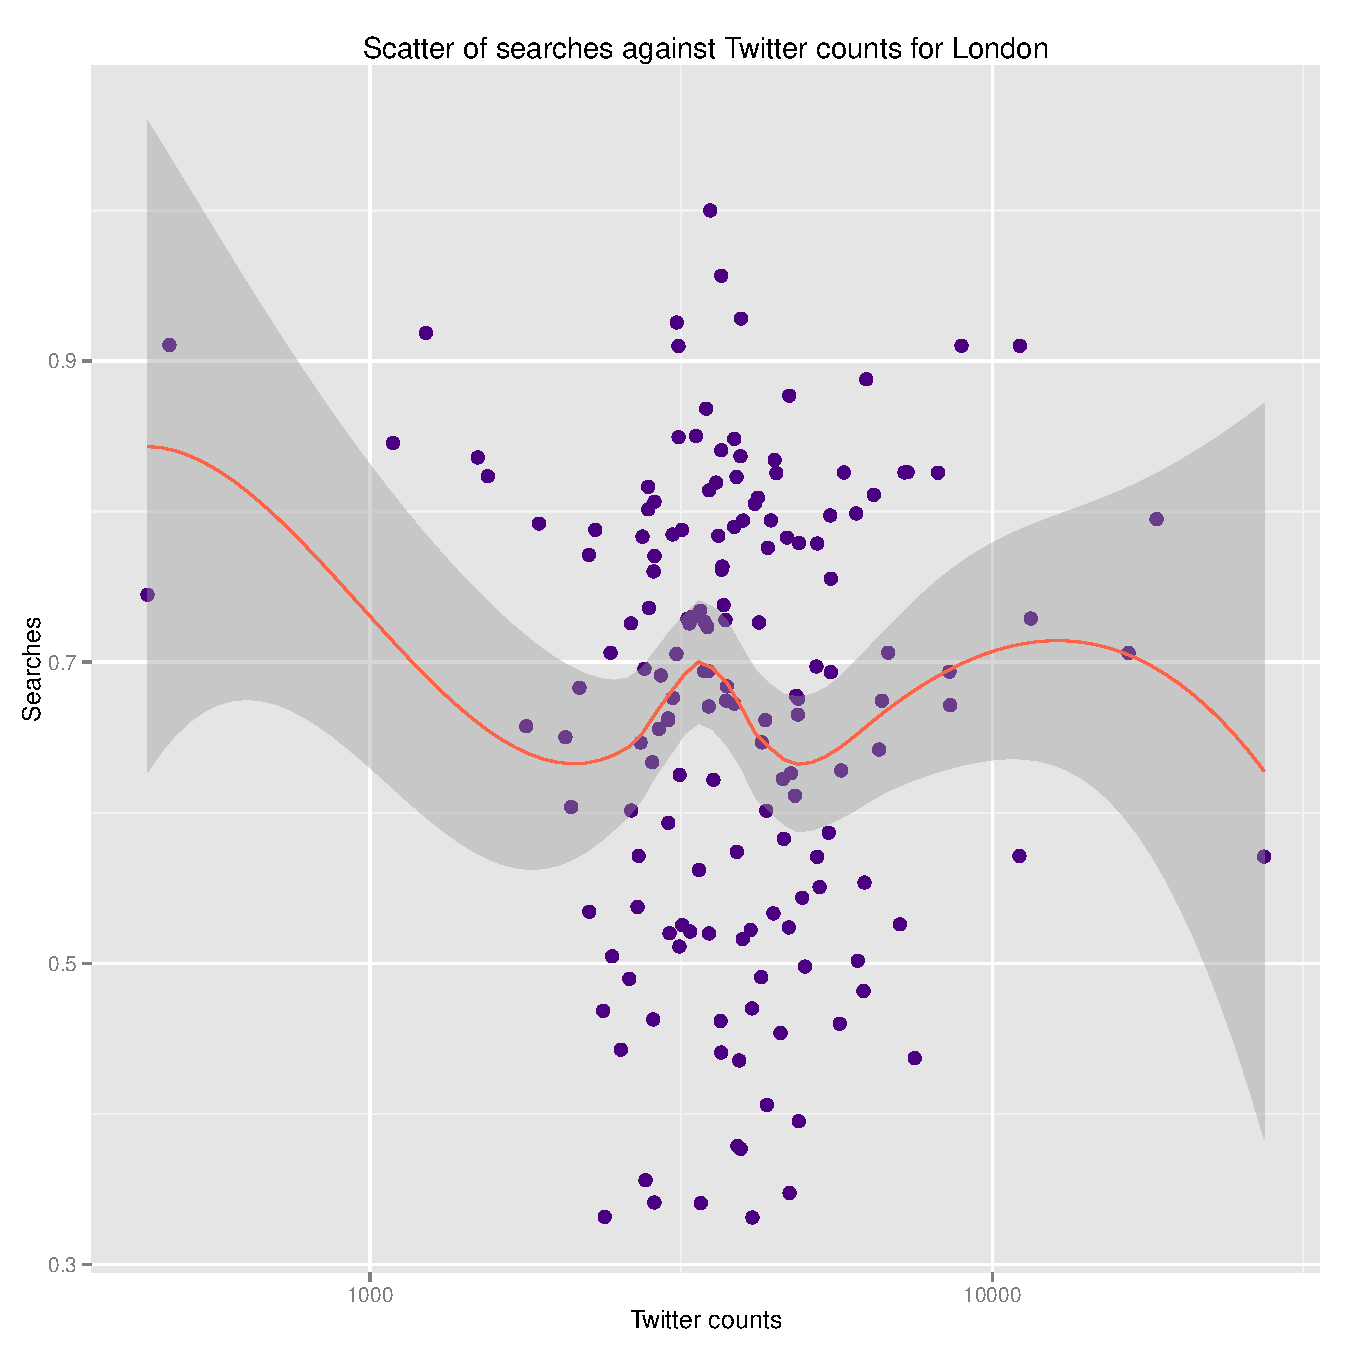
\includegraphics[width=\textwidth]{London}

There is definitely a relationship, even though not perfectly linear.

We can observe that there is a well defined cluster where the twitter counts are big and the corresponding searches are relatively big as well. We can't say with great certainty that those two are perfectly correlated, because correlation does not imply causation. So what we needed to do was to delve even further and build a model that would work with those.

%So we can certainly say that those variables are correlated, but the outliers push the coefficient down quite a significant amount. The interesting part of this scatter plot for us is the top right corner. We are interested in those abnormal Twitter counts, which correspond to high number of redirects. Another interesting thing to explore would be to see if we correlate the mentions on the social network with the redirects from the next day. That will assume a certain lag factor, which is reasonable as sometimes an event should not effect the redirect counts till the next day when it's picked by all the major media. 

Paris was one of the most popular destinations so it was quite interesting to see what the relation is there. The Pearson test yields the following values for Paris:
\begin{quotation}
In [24]: r\_value, p\_value

Out[24]: (-0.25, 0.0047)
\end{quotation}
\newpage
And here is the scatter plot:

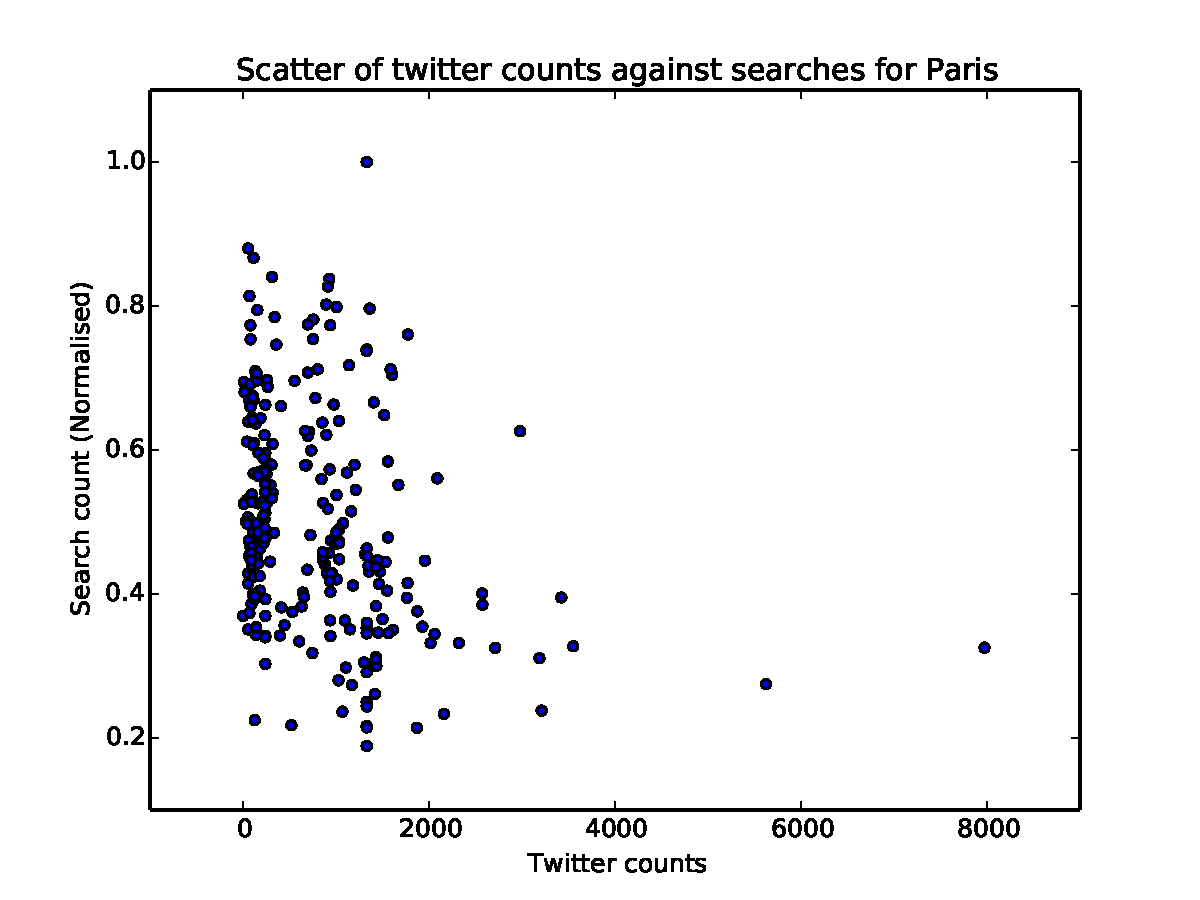
\includegraphics[width=\textwidth]{Paris}

Here we do see that indeed the correlation is relatively small and negative. 

As we can see each of the different cities shows a different behaviour. The implications of that are that the approach we take to building the model must be more versatile - we will aim to build one model for the overall numbers and models on a per city basis.

\section{Cleansing the data}

As mentioned, every time you depend a few external data source there will be some problems with the data, caused by several things. 

In this project there were a couple of major sources of problems:
\begin{enumerate}
\item The script that collects data from the Streaming API.
\item The searches data coming from Skyscanner being incorrect or partial - not spanning the full date range.
\end{enumerate}

The dates with incomplete data or missing data altogether can seriously impact any regression or statistical test, so it was vital to tidy up the data set by backfilling it. I applied the Last 4 Fridays forecasting algorithm mentioned in the following chapter in order to make the dataset more consistent and easier to work with. 

The interesting part was that it completely change the results from the test. For London the values returned by the Pearson test are now:

\begin{quotation}
In [23]: r\_row, p\_value

Out[23]: (-0.23, 0.02)
\end{quotation}

That is quite interesting and it has a lot of implications on the models we will use afterwards to correlate the two variables. 
We might have to add a certain "lag" factor to this, which will offset the tweets by correlating the numbers extrapolated from Twitter with the numbers and match them against searches from the following day.

%\section{Top features} 

%The idea here is to extract the top N features from the tweet and use them in the logistic regression model that we will build to predict the search counts. I plan on working on this in the next couple of weeks.


\chapter{Models}
\label{chap:model}

\section{The baseline model}
\label{sec:baseline}

The baseline model for predicting the number of redirects Skyscanner has on a daily basis is called Last 4 Fridays. 
It works in the following way:
\begin{enumerate}
\item We want to predict the number of redirects/searches for this Friday.
\item We take the number of redirects/searches Friday from last week, the week before, etc, until we have the counts form the previous 4 weeks for the corresponding day.
\item We then assign weights to those 4 numbers and assign weights - the most recent one will get the highest weight, the one after about a half and so on. The exponential weighting scheme captures short term seasonality.
\end{enumerate}

This model was tested out against more complex models like ARIMA and Autoregressive Vector Methods and it performed really well, but unlike the others it was many times simpler to program and maintain.

\section{Last 4 Fridays + Twitter Counts}

The first model I build was not a radical new approach, but rather an increment on the previous one.

I generated a list of tuples which contained the following information:
\begin{itemize}
\item Twitter count for the place - how many times it was mentioned in conjunction with a travel term.
\item Same day of the week from last week
\item Same day of the week from 2 weeks ago
\item Same day of the week from 3 weeks ago
\item Same day of the week from 4 weeks ago
\end{itemize}

What this is is a version of Last 4 Fridays which now has Twitter Counts. Instead of using the exponential weights from the previous algorithm I let LASSO determine their weights.
With LASSO I had weights for each of the 272 cities. After measuring the RMSEs for the L4F algorithm and expanded version with Twitter Counts the former performs better on 193 of the 272 cities. In the top 10 L4F+Twitter performs better on 2 out of 10. 

Dublin which is in the 4th spot in terms of volumes is quite interesting. I plotted out the counts against searches just to see how it looks:

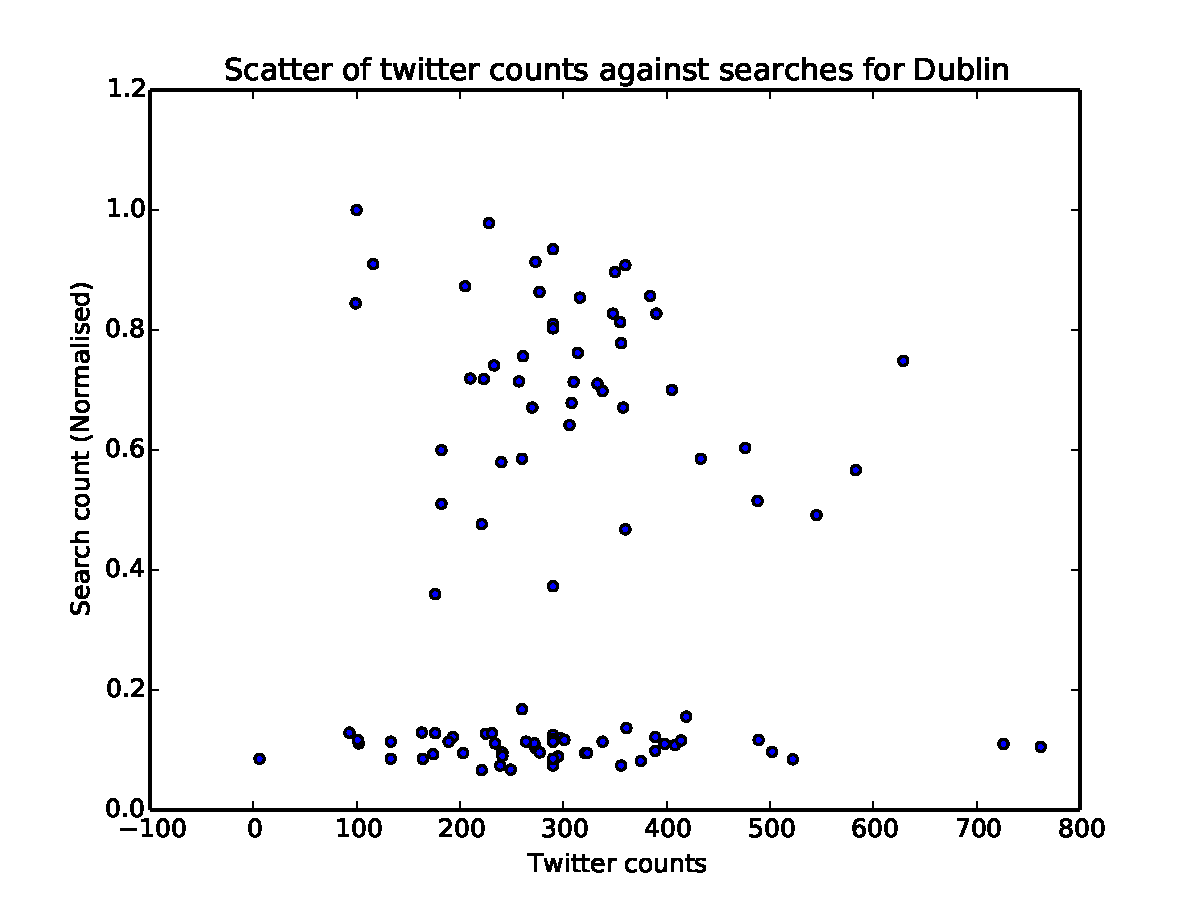
\includegraphics[width=\textwidth]{Dublin}  

\newpage
\section{Results}

And here are the results for the top 10 destinations by volume (they have the highest RMSEs).

\begin{tabular}{ l | r | r }
City	& RMSE L4F+Twitter &RMSE L4F \\
\hline
London & 3335.869525 & 3160.05886 \\
Paris	 & 939.1057276 & 921.6785638  \\
Barcelona & 920.6831066 & 897.6473097  \\
Milan & 760.3436591 & 760.9286718  \\
Rome & 710.7052517 & 705.8388511  \\
Manchester & 574.8431422 & 572.4116201  \\
Dublin & 514.584231	 & 527.884409  \\
Amsterdam & 550.2254781 & 516.2054596  \\
Tenerife & 544.6187529 & 502.0270723  \\
Moscow & 499.1803266 & 495.2139406  \\
\end{tabular}


This is quite a good start considering the fact that all the weights were automatically determined by the LASSO algorithm and the fact that I have only about 130 data points so far (130 days).

\section{Future improvements}

The next on the list is to expand the feature set with more features from Twitter such as:


\begin{itemize}
\item Specific words.
\item Trending event or not.
\item Investigate whether sentiment will be useful here.
\end{itemize}

With those I'll be able to better the model and reduce the RMSE across the whole board and hopefully beat the current prediction algorithm for more than 80\% of the examples.


\chapter{Future work}
\label{chap:future-work}


%\chapter{Timeline}

%The timeline for the next 3 months is the following:
%\begin{enumerate}
%\item Better the existing model and continue with the tests. .
%\item Add more features to the set of inputs.
%\item Work on both approaches:
%\begin{itemize}
%\item Explain spikes in searches by looking at historical tweet data
%\item Or try to predict the spikes in the first place
%\end{itemize}
%\item Final draft done by mid-March.
%\item Submit dissertation the final week of March.
%\end{enumerate}

\begin{thebibliography}{10}

\bibitem{seqcap}
	BBC, \emph{Sequoia Capital investment values Skyscanner at \$800m}, \\
	{\url{http://www.bbc.co.uk/news/uk-scotland-scotland-business-24380126}}

\bibitem{code}
	Stefan Sabev, Code for Inf Project,\\
	{\url{https://github.com/SSabev/HonsProject/}}
	
\bibitem{lasso}
	Wikipedia, \emph{Lasso (statistics)}, \\
	{\url{http://en.wikipedia.org/wiki/Lasso_(statistics)#Lasso_method}}
	
\bibitem{TwitterNewsWire}
	Twitter, \emph{Twitter as a news-wire}, \\
	{\url{https://blog.twitter.com/2008/twitter-news-wire}}

\bibitem{TwitterResearch}
	Twitter Research,
	\emph{A collection of publications using Twitter data}, \\
 	{\url{https://sites.google.com/site/twitterresearch09/twitter-papers}}

\bibitem{Miles}
	Miles Osborne, \emph{Social media papers}, \\
	{\url{http://homepages.inf.ed.ac.uk/miles/sm-papers.html}}
	
\bibitem{Petrovic2012}
	Sasa Petrovic
  	\emph{Real-time Event Detection in Massive Streams 2012} ,\\
	School of Informatics, University of Edinburgh \\
	{\url{http://homepages.inf.ed.ac.uk/s0894589/petrovic-thesis.pdf}}

\bibitem{twitstock}
	Johan Bollen, Huina Mao and Xiao-Jun Zeng, \\
	\emph{Twitter mood predicts the stock market}, \\
	{\url{http://arxiv.org/pdf/1010.3003v1.pdf}}

\bibitem{twitnfl}
	Shiladitya Sinha, Chris Dyer , Kevin Gimpel, and Noah A. Smith, \\
	\emph{Twitter mood predicts the stock market}, \\
	{\url{http://arxiv.org/pdf/1010.3003v1.pdf}}

\bibitem{twitflu}
	Michael J. Paul and Mark Dredze,  \\
	\emph{You Are What You Tweet: Analyzing Twitter for Public Health}, \\
	{\url{http://www.cs.jhu.edu/~mdredze/publications/twitter_health_icwsm_11.pdf}}

\bibitem{twitpoll}
	Brendan O?Connory,  Ramnath Balasubramanyany, Bryan R. Routledgex, Noah A. Smith, \\  
	\emph{From Tweets to Polls: Linking Text Sentiment to Public Opinion Time Series}, \\
	{\url{http://www.cs.cmu.edu/~nasmith/papers/oconnor+balasubramanyan+routledge+smith.icwsm10.pdf}}

\bibitem{dija}
	Wikipedia, \emph{Dow Jones Industrial Average}, \\
	{\url{http://en.wikipedia.org/wiki/Dow_Jones_Industrial_Average}}

\bibitem{opfind}
	OpinionFinder, \\
	{\url{http://mpqa.cs.pitt.edu/opinionfinder/}}
	
\bibitem{granger}
	Granger causality, \\
	{\url{http://en.wikipedia.org/wiki/Granger_causality}}

\bibitem{sofnn}
	Gang Leng, Girijesh Prasad, Thomas Martin McGinnity
	\emph{An on-line algorithm for creating self-organizing fuzzy neural networks}
	{\url{http://www.sciencedirect.com/science/article/pii/S0893608004001698}}
  
\bibitem{Hamletkdd03}
 	Etzionni, Tuchinda, Knoblock and Yates, \emph{To Buy or Not to Buy: Mining Airfare Data to Minimize Ticket Purchase Price}, 2003, \\
  	{\url{http://knight.cis.temple.edu/~yates/papers/hamlet-kdd03.pdf}}
	
\bibitem{ijcai}
	William Groves and Maria Gini, \emph{Optimal Airline Ticket Purchasing Using Automated User-Guided Feature Selection} \\
	{\url{http://ijcai.org/papers13/Papers/IJCAI13-032.pdf}}

\bibitem{samplestream}
	Twitter Sample Stream, \\
	{\url{https://dev.twitter.com/docs/api/1.1/get/statuses/sample}}

\end{thebibliography}

\end{document}
